\documentclass[12pt]{article}
\usepackage{amsmath,amssymb,amsthm}
\usepackage{graphicx,mathabx}
\usepackage{xcolor}
\usepackage{tikz}
\usepackage{placeins}
\usepackage{lipsum}
\usepackage[shortlabels]{enumitem}
\usepackage{placeins}
\usepackage[makeroom]{cancel}
\usepackage{mathrsfs}
\newcommand\tab[1][1cm]{\hspace*{#1}}
\def\blankpage{%
      \clearpage%
      \thispagestyle{empty}%
      \addtocounter{page}{-1}%pdf
      \null%
      \clearpage}
\begin{document}
\title{TCSS 343 - Week 7}
\author{Jake McKenzie}
\maketitle
\noindent\centerline{\textbf{Graph Algorithms and some Greedy Algorithms}}\\\\\\\\\\\\\\\\
\begin{center}
    ``Finding a needle in a haystack is actually quite easy. It's finding a very specific piece of hay in a haystack that happens to be hard." \\$\dots$\\ Avi Wigderson
\end{center}
\begin{center}
    ``People say nothing is impossible, but I do nothing every day'' \\$\dots$\\ Winnie-the-Pooh
\end{center}
\begin{center}
    ``It is not enough to be in the right place at the right time. You should also have an open mind at the right time." \\$\dots$\\ Paul Erd\H{o}s
\end{center}
\newpage
\noindent There are $n$ trading posts numbered $1$ to $n$, 
as you travel downstream. At any trading post $i$, you can rent 
a canoe to be returned at any of the downstream trading posts $j > i$. 
You are given a cost array $R(i,j)$ giving the cost of these rentals for 
$1 \leq i \leq j \leq n$. We will have to assume that $R(i,i) = 0$ and $R(i,j) = \infty$ 
if $i > j$. For example, withn = $4$, the cost array may look as follows: The rows are the 
sources ($i - s$) and the columns are the destinations ($j$’s).\\
\centerline{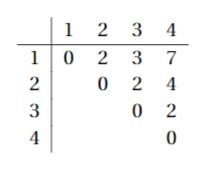
\includegraphics[scale = .8]{posts.jpg}}\\
The problem is to find a solution that computes the cheapest sequence of rentals taking 
you from post $1$ all the way down to post $n$. \\\\
0. State the input and output conditions for this problem as precisely (tidy) as possible.\\\\\\\\\\\\\\\\\\\\
1. Why do greedy algorithms fail to solve this problem?
\newpage
\noindent 2. Modify Kruskal's algorithm to find the maximum spanning tree.\\
\fbox{
    \parbox{10cm}{
      KRUSKAL \\
      
      $T = \emptyset$ \\
      FOR each vertex $v \in V$ {\sc Make-Set}($v$)
      
      Sort edges of $E$ in increasing order by weight \\
      FOR each edge $e=(u,v) \in E$ in order DO
      \begin{itemize}
      \item[] IF {\sc Find-Set}($u$) $\neq$ {\sc Find-Set}($v$) THEN
	\begin{itemize}
	\item[] $T = T \cup \{ e \}$
	\item[] {\sc Union-Set}($u,v$)
	\end{itemize}
      \end{itemize}
  }}
  \newpage
 \noindent 3. Modify Prim's algorithm to find the maximum spanning tree.\\
  \fbox{
    \parbox{10cm}{
      PRIM(r)\\
      
      For each $v \in V$ DO
      \begin{itemize}
      \item[] {\sc Insert}($PQ,v,\infty$)
      \end{itemize}
	  {\sc Decrease-Key}$(PQ,r,0)$ \\
	  WHILE $PQ$ not empty DO
          \begin{itemize}
          \item[] $u$ = {\sc Deletemin}($PQ$)
	  \item [] (output edge $(u, visit(u))$ as part of MST)
          \item[] For each $(u,v) \in E$ DO
            \begin{itemize}
            \item[] IF $v \in PQ$ and $w(u,v) < $ key($v$) THEN
            \item[] ~~~~visit[$v$] = $u$
            \item[] ~~~~{\sc Decrease-Key}($PQ,v,w(u,v)$)
            \end{itemize}
          \end{itemize}
  }}
\newpage
\noindent With this problem I want to present to you an orientation where the 
greedy algorithm fails and when the algorithm succeeds.\\\\
Imagine we have a wizard that knows a few spells. 
Each spell has 3 attributes: Damage, cooldown time, and a cast time. \\\\
\textbf{Cooldown time:} the amount of time (t) it takes 
before being able to cast that spell again. 
A spell goes on ``cooldown" the moment it begins casting.\\\\
\textbf{Cast time:} the amount of time (t) it takes 
to use a spell. While the wizard is casting 
something another spell cannot be cast and 
it cannot be canceled. \\\\
\textit{The question is:} \textbf{How would you maximize damage 
given different sets of spells?} \\\\
It is easy to calculate the highest damage per cast 
time. But what about in situations where it is better 
to wait then to get ``stuck" casting a low damage 
spell when a much higher one is available...for example consider
the two spells and two actions you can do on those spells totally four actions:\\\\\\
Chill Touch: $100$ damage at a rate of $1$ second per cast with a $10$ second cooldown. \\\\
Mage Hand. $10$ damage at a rate of $4$ second per cast with a $0$ second cooldown.\\\\
Optimal action ordering $\Sigma =\{$Chill Touch, Mage Hand, Wait, Repeat$\}$\\\\
4. Given an arbitary amount of time $t$ what is the maximum amount of spells
we can cast $S$ for some arbitary period?
\newpage
\noindent Now imagine that there is one spell, henceforth called the Eldritch Blast, 
which does a very, very large amount of damage much more than the two current spells you have, has $0$ casting time, and has 
some positive cooldown $n$. If all the other spells do much less damage than the 
Eldritch Blast, it will clearly be optimal to cast the Eldritch Blast every n seconds and 
then optimize the cooldown time with the weaker spells.\\\\
5. Why does the greedy algorithm work in this case?\\\\\\\\\\\\\\\\\\\\
Now, assume all the other spells also have cooldown $n$. 
If one optimizes a given n-second downtime with these spells, 
then the same spell-sequence will also be possible in the next 
$n$-second downtime, and so we can assume the solution is $n$-periodic.\\\\
6. Why does the greedy algorithm fail in this case?\\\\\\\\\\\\\\\\\\\\ 
\newpage
\noindent 7. Consider the following undirected, weighted graph:\\
\centerline{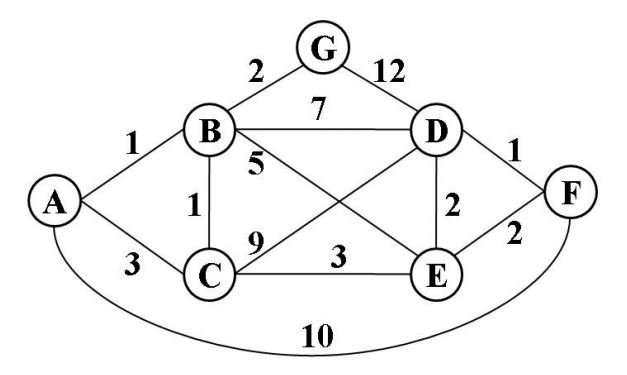
\includegraphics[scale = .7]{graph.jpg}}\\
Step through Dijkstra’s algorithm to calculate the single-source shortest 
paths from A to every other vertex. Show your steps in the table below. 
Cross out old values and write in new ones, from left to right within each 
cell, as the algorithm proceeds. Also list the vertices in the order which 
you marked them known. Finally, indicate the lowest-cast path from node A 
to node F.\\
\textbf{Known vertices:} $\rule{1cm}{0.15mm}$ $\rule{1cm}{0.15mm}$ $\rule{1cm}{0.15mm}$ $\rule{1cm}{0.15mm}$ $\rule{1cm}{0.15mm}$ $\rule{1cm}{0.15mm}$ $\rule{1cm}{0.15mm}$\\
\textbf{(in order marked known)}\\
\centerline{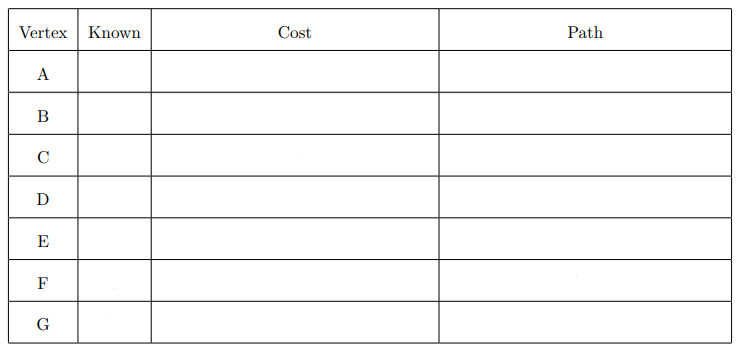
\includegraphics[scale = 2]{table.jpg}}\\\\
\textbf{Lowest-cost path from A to F:} $\rule{7cm}{0.15mm}$
\newpage 
\noindent 8. Consider the following directed, weighted graph:\\
\centerline{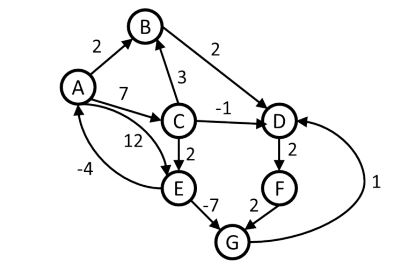
\includegraphics[scale = 0.7]{graph3.jpg}}\\
Even though the graph has negative weight edges, step through Dijkstra’s algorithm to calculate
\textit{supposedly} shortest paths from A to every other vertex. Show your steps in the table below.
Cross out old values and write in new ones, from left to right within each cell, as the algorithm
proceeds. Also list the vertices in the order which you marked them known.\\\\
\textbf{Known vertices:} $\rule{1cm}{0.15mm}$ $\rule{1cm}{0.15mm}$ $\rule{1cm}{0.15mm}$ $\rule{1cm}{0.15mm}$ $\rule{1cm}{0.15mm}$ $\rule{1cm}{0.15mm}$ $\rule{1cm}{0.15mm}$\\
\textbf{(in order marked known)}\\
\centerline{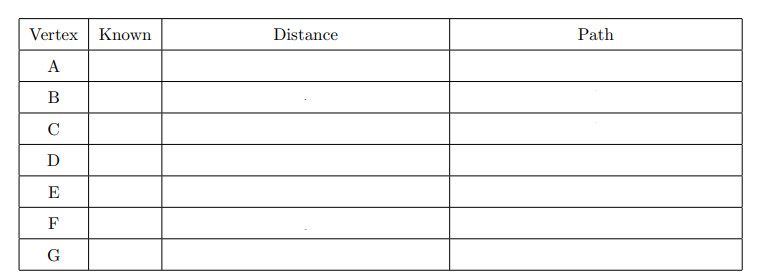
\includegraphics[scale = 2]{table2.jpg}}\\
9. Dijkstra’s algorithm found the wrong path to some of the vertices. For just the vertices where
the wrong path was computed, indicate both the path that was computed and the correct path.\\\\\\\\
A. What single edge could be removed from the graph such that Dijkstra’s algorithm would happen
to compute correct answers for all vertices in the remaining graph?
\end{document}